\documentclass[11pt,a4paper]{article}
\usepackage{fullpage}
\usepackage{graphicx}
\setlength{\parskip}{0.5em}
\begin{document}
\author{Muhammad Zaheer}
\title{Smart Grids -- An overview}
\maketitle

\section{Introduction}
The electric power grid is considered to be one of the greatest engineering achievement of the 20\textsuperscript{th} century.Since the first electricty network set up by Thomas Edison, electricity became one of the main drivers in economic progress of the country. There is a causal relation between the GDP and the electricity consumption in a country\cite{Jumbe200461}.The electricity industry was largely operated by government owned companies and were vertically integrated. The companies used to manage the entire energy value chain and had a monopoly over a given area where they were licensed to operate. Initially, this led to a stable environment for the power industry to develop and soon it was a stable industry.

However, the whole industry has been affected by the recent changes brought about by the regulatory authorities. First, the whole electricty sector was directed to be unbundled and electricity markets were introduced to increase competiveness and reduce the electricity price fot the end consumer. The unbundling of the sector led to the creation of separate entities that were responsible to the generation, transmission and distribution of power. Next, the climate change issue has forced the power industry to make a concerted effort in increasing the quota of power generation from renewables and decreasing the generation of power from fosil fuel power plants. Lastly, the Fukushima incident(2011) in Japan resulted in laws to shut down the nuclear plants all over the world. This made life very difficult for the people involved in operation and management of the power system.This meant that they had to be prepared for operating the sytem without the generation mix that contributed to the base load demand.  A characteristic of the fossil fuel/nuclear based power plants was that they were cheap and controllable i.e. we could increase/decrease the power generation as and when needed to match the varying load demand. For renewable energy, we have no control over the dispatch of power. Hence,such a directive has put a lot of pressure on the industry as they need to operate the power system which has a lot of variablitlity on the generation side.

Let us look at some of the challenges facing the electric power industry today and how smart grid technologies will help in solving these issues.

\section{Increase in grid capacity}
The purpose of the power grid is to provide a path for the flow of generated power to the connected load. A general rule of thumb was that electricity demand will always keep increasing and hence huge investments in the generation, transmission and distribution of power was always required to cater to the future load on the system. World population is set to grow at a rate of around 1.25\% and is pegged to be close to 9 billion by 2030. This factor coupled by the economic growth will result in the growth of electricity consumption per capita. Hence, there is a need for an increase in grid capacity to serve the future load on the system. The problem arises wherein, the return on investment period on the transmission and distribution grid is close to 30 years and it does not make business sense to invest large amounts when the future of the industry is changing very rapidly. The smart grid technologies allow for increasing the grid capacity without much risks.

\subsection{FACTS and HVDC}
Power flow in the transmission and distribution grid is governed by Kirchoff's voltage and current law. Hence, given a network topology we cannot control how much power flows through a given transmission line. The advent of power electronics have helped change this. Flexible AC Transmission Systems(FACTS) and High Voltage DC (HVDC) transmission has been made largely possible by the development of power electronic devices and circuit. These power electronic circuits helped in the operation of the power system very much.

For the FACTS, there are two types of components. One type is the switched components that are connected to the transmission line and change the characteristics of the particular line i.e. decrease/increase the impedance of the line thereby controlling the flow of power. An example for this kind of a device is the Thyristor controlled Reactor(TCR). This device is connected to a transmission line and by varying the signal to the device, we can control the reactive power flow in the line which in turn frees up the path for more flow of active power. Other type is the devices based on the Voltage Source Inverter(VSI). These devices work on the principle of injecting a voltage in series with the line and by changing the injected voltage, one can control the real/reactive power control and also voltage at the bus. An example of such a device is the Synchronous Static Compensator(STATCOM)\cite{g2001understanding}.

In HVDC, the major components in the system is the rectifier/inverter. These devices are responsible for the conversion of AC into DC and vice versa. In the HVDC system, the power flow depends on the voltage at a given bus and it is controlled by the signal given to the rectifier/inverter. The advantage of this system is that there is only resistive loss and controllability is very high. Also, this kind of a system helps in interconnecting two asynchronous AC systems and can help in providing stability to both the systems. The only drawback with this technology is its high investment cost which makes it economically feasible only for long transmission.

These technologies help in utilizing the grid much more effectively and the investment required and the time taken to set it up is less compared to installing new transmission lines.

\subsection{Dynamic Line Rating}
This concept is an example of how the grid capacity can be increased very much without much effort. In a transmission line, the conductors are rated for higher load than necessary for reliable operation. Also, the power flow through the line is always kept below a specific margin so that the line does not get damaged. One of the main reasons for this is that when the load on the line increases, the sag increases which, by law, can go beyond a certain level as this can cause damage to the surroundings. However, if weather conditions permit, we can go to higher load without violating the sag condition and hence can use the available transmission capacity much better than before.

Elia has worked with the University of Liège and Ampacimon for several years on a technology that enhances the transmission of energy over high-voltage lines under specific weather conditions (i.e. when it is windy and cold). Elia is the first transmission system operator to use this technology on international lines.The decision to install this device on the southern and northern borders of Belgium is part of the various initiatives taken by Elia to deal with the risk of power shortages. The small device will be placed on the eight border lines, boosting physical flows by 10 to 15\% in the event of low temperatures, according to the force and speed of the wind as well as other specific conditions\cite{elia:2014}.

\section{Influence on the reliability of  the grid}
Power system reliability is paramount in recent times owing to the customer's demands and also due to the fact that in case of non-compliance a very large amount of people are affected and the damages due to this can run into millions of dollars. An example for this case is the blackout that occured in North America in 2003. The blackout occurred in parts of North-eastern and Midwestern United States that resulted in lack of power for almost a day and in some parts for more than a day. The number of people affected due to this was closely 20 million people. Post-mortem analysis showed that the blackout occured due to a bug in the control software that led to a race condition and hence did not alarm the authorities of the event\cite{pmudeploy2012}.

\subsection{Wide Area Measurement Systems}
Blackouts and/or cascading failure have impacted the lives of the customer gravely and also led to economic loss for businesses. It is necessary to anticipate such events and prevent them from occuring ever. One way to tackle this is to deploy a Wide area Measurement System(WAMS). A common thread in the causes for such blackouts was found to be lack of situational awareness of the operators reponsible for the power system. This can be traced back to the fact that the power system data is managed by the Supervisory Control and Data Acquisition(SCADA) system. This system receives data from measuring point approximately every 10 seconds and the data typically measured is the voltage, current and power levels at a substation. This data while being vital arrives too slow and too late given that once the data arrives, it needs to be validated and then processing of this data is done before we can have any useful information. Another issue with the data is the sampling time i.e. the data collected from different measuring nodes is not sampled at the same time and hence it does not gives us a snapshot of the power system accurately.

To tide over this problem, Transmission system Operators(TSO) have started to deploy Phasor Measurement Unit(PMU) across the entire national grid. A PMU is a device which does simultaneous sampling of voltage and current angles and the data is timestamped against a GPS clock which is synchronized across all devices and is transmitted every 1 second. The data thus received gives the operator a better view of the entire power system and what actions need to be taken to manage outages in case it occurs\cite{pmusitu2010}. The challenge with such a deployment is the communication infrastructure that is required to transfer such data as it requires a high bandwidth whereas conventional communication in the power industry has been happening over low bandwidth networks. This requires an investment in new infrastructure and business cases are being drawn up to answer these questions. An example of a utility wide scale deployment of PMUs can be found in the document\cite{usoutage2004}.

\section{Increase in efficiency of the grid}
Increasing the efficiency of the grid in other words means minimizing the losses in the system. Losses in the system occur mainly from the $I^{2}R$ losses. While we cannot reduce the resistance of the line until we replace it with another line, we can reduce the current flowing in the line by increasing the voltage level at which the grid is operating. Countries like India and China are looking at Ultra High Voltage DC(UHVDC) Transmission where voltage levels are greater than 400kV. ABB is implementing a multi-terminal UHVDC link of 800kV in India that connects the Northern part of India to the Nort-eastern part which will enable a transmission capacity of 8000MW from the Northeast to the central part of India\cite{abbhvdc2014}. In this project, the losses are estimated to be around 6\% which compared to the T\&D losses in India is around 12-15\%.

There are also some projects that are looking at High Temperature Superconductor(HTS) installations but we are still some years behind the actual implementation.

\section{Making the energy value chain sustainable}
To build a electricty grid that is sustainable, we need to utilize as much of renewable energy as possible. However, to satisy this condition the electricity generation needs to become decentralized as the energy resources are distributed over a vast area. This requires a change in the network topology to accomodate distributed generation. Conventionally, the electric power grid was built to deliver power from the generators to the load wherein the generation happened is centralized areas far away from the load centers.

With distributed generation(DG), customers are not only consumers but also producers of energy hence coining a new buzzword in the industry 'prosumers'. To facilitate this, the grid needs to become bidirectional and meters will have to be replaced with net metering. Since, most of the power produced will be from the solar PV panels, their interface to the grid will be a power electronic converter which is known to pollute the power system with harmonics. Hence,strict regulations will need to be drawn up of the requirements for injecting the power into the grid. Also, protection schemes will have to redesigned to allow bidirectional power flow in the grid. The figure~\ref{fig:pvgrid} below shows an example of connecting a residential PV panel to the grid through a bidirectional power meter. With demand response mechanism, the utility can communicate with the meter and control appliances at the customer's home.
\begin{figure}[h]
  \centering
  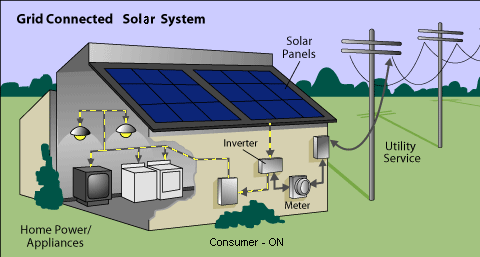
\includegraphics{gridpvtie.png}
  \label{fig:pvgrid}
  \caption{An example of PV panel and grid interfacing}
\end{figure}


Another important measure that can help make the energy system more sustainable is demand response(DR). Earlier, the power system was operated with the philosophy that load is uncontrollable and hence we need to control the generation to maintain balance. However, with the advent of communications, we can set up a platform wherein the operators can notify the customer of an imbalance in the grid and signal the customer to reduce/increase the load to maintain the balance. Such a measure can help power systemoperators in a huge way. With this, they can reduce their investments in peak power production and capacity reserves. All these conditions can be satisfied only if the customer is exposed to Time of Usage (ToU) tariff i.e. the basic philosophy is that we enable the customer to use more energy during off-peak periods and vice versa. This mechanism will help in reducing the diversity factor in the power system. Also, such control will alow the operators to counteract the variability of the renewable energy sources which can lead to stability issues if not managed properly.

Energy Storage is another important aspect in making the grid more sustainable. A lot of work has been done in increasing the power/energy density of batteries and we will be seeing grid-level storage projects soon. A clear advantage of this technology is that it can absorb the variabibilty of the renewable energy sources and deliver power when there is shortage. Pumped hydro plants have been used for a long time for energy storage but with development of electric vehicles(EV), a huge boost has been given to development of batteries and this in turn will help in managing the dynamics of the grid better.

\section{Flexibility in Electricity markets}
Unbundling of the traditional utilities and creation of a electricity market has changed the way a power system is managed and operated. Before the unbundling process, the utility was involved in generation, transmission and distribution of electric power and therefore the electricity tariff depended upon how much the utility was focussed in bringing the costs down. In other words, there was a monopoly in a region by the utility and the consumer had no choice but to pay at whatever rate he was asked to. However, unbundling has created separate entities for the different aspects i.e. separate independent companies for generation, transmission and distribution of electric power. This has encouraged competition as the customers have a choice as to from whom they want to procure power and to whose network they want to stay connected to. This has led to reduction in electricty prices.

The electricity market has transactions that can be divided into three categories viz., short-term, medium-term and long-term contracts. Apart from these, a number of markets have been created to satisfy different requirements. In the Day-ahead market, one can buy/sell power for the next day and in the intra-day market operates for power transactions for the same day. The intra-day market is heavily influenced by the real-time network conditions and hence can be very expensive to buy on this market.

The challenges that a TSO usually faces is congestion management of the power grid and this issue becomes relevant when there is shortage of power in one region and surplus power from another region cannot be imported due to congestion in the lines. This makes scheduling of power and contract agreements very complex. Some of the technical developments that can help ease this is integrating FACTS device into the existing power grid. Another solution is to use the PMU data to visualize the state of the power system and take informed decisions on stability issues due to such congestion in the lines.
\section{Impact of Electric Vehicles on the grid}
Climate change has resulted in governments framing policies which are favourable to reduce greenhouse gas emissions. One of the action points is to reduce the use of fossil fuel in any activity. This has led to electric vehicles becoming popular in recent times. The price for an electric vehicle is still very high compared to gasoline vehicle but due to tax breaks from the governement, the electric vehicle is getting public acceptance. Even though the electric vehicle has not gained wide acceptance, it is very clear that it will replace a large part of the passenger cars. Hence, it is the right time to analyze its impacts and take appropriate step to accomodate it into the electtricity grid.

Wide adoption of electric vehicles will result in increase in load demand due to charging of batteries. Now, the increase in energy consumption will be around 10-15\% of present total energy consumption. However, the generation capacity needs to increase by more than 100\% to cater to this load. However, if we manage the charging of vehicles properly, the increase in grid capacity can be limited to around 20\%. This can be done by using ToU tarrif such that charging of vehicles can be done during off peak hours so that the stress on the power system is compariticely less\cite{cao2012optimized}.

Battery charging technologies will decide on the increase in grid capacity and hence we need to analyze the different strategies . Fast charging is regarded to be the answer for limited-range issue of electric vehicles i.e. one could charge their batteries to 80\% in half an hour but the charger has a power rating of 120kW which can load the power system too much if a lot of them is switched on simultaneously. Slow charging can be done which takes a lot of time to charge but the power rating is around 10kW which might not load the system that much. Special charging infrastructure will be required to facilitate fast charging as normal household outlets will not support drawing such magnitude of power.

Another important impact of electric vehicles will be in the area of energy storage. A fleet of battery electric vehicles has the same amount of storage capacity as required for grid level storage. Demand Response mechanism can be employed for supplying and consuming energy so as to help balance the generation and the load.

\bibliography{report}
\bibliographystyle{plain}
\end{document}
